% Chapter 1: Words That Won't Hold Still

\chapter{Words That Won't Hold Still}

On March 2, 2008, at 3:13 in the morning, I got an email from Rodney Huddleston about a word he didn't understand.

The time stamp is misleading~-- Huddleston was writing from Australia, where it was a reasonable hour. But there's something fitting about the image of a linguist awake in the dark, wrestling with a single word. The word was \mention{otherwise}. I had asked him whether there were grounds for treating it as a preposition rather than an adverb. His reply:

\begin{quote}
I'm not proud of the adverb analysis, or confident about it, and don't intend it to cover all uses. Its classification is quite a puzzle. Dictionaries have it as adverb and adj (\mention{the truth is quite otherwise}) and some also as conjunction. There is something to be said for a prep analysis, which might cover adjunct and predicative complement uses. But I don't know how to handle \mention{this suggests otherwise} or \mention{the correctness or otherwise of the proposal}.
\end{quote}

Huddleston was not a careless analyst. He was the lead author of \textit{The Cambridge Grammar of the English Language} \citep{huddleston2002}~-- 1,860 pages, seventeen years in the making, the most comprehensive descriptive grammar of English ever produced. If anyone knew what \mention{otherwise} was, it should have been him.

But he didn't. Not because he had missed something. Because the word wouldn't hold still.

\bigskip

This book is about what that puzzle reveals.

The natural reading is that \mention{otherwise} is simply a hard case~-- an outlier, a word with an unusual history, a problem for specialists. Every grammar has its edge cases. You note them, flag the uncertainty, and move on.

But \mention{otherwise} is not alone. Each of the following behaves as if it were built from a different blueprint than the one our categories assume:

\mention{Cattle} takes plural agreement (\mention{the cattle are grazing}) but has no singular. You can say \mention{many cattle} or \mention{three cattle}, but not \mention{a cattle} or \mention{one cattle}. Yet it readily functions as a modifier in compound nouns like \mention{a cattle ranch}, a position usually reserved for singulars (\mention{a toothbrush}, not \mention{*a teethbrush}). The usual singular--plural paradigm simply doesn't apply. And it has been this way for centuries~-- not drifting toward regularity, not acquiring a singular, just sitting there being strange.

\mention{The} marks definiteness~-- or so the textbooks say. But \mention{go to the hospital} doesn't pick out a particular hospital. \mention{The tiger is endangered} doesn't refer to any individual tiger. These aren't rare or marginal uses; they're ordinary English, and they're well-known problem cases precisely because the standard definition of definiteness~-- that the referent is identifiable to the hearer~-- fails to cover them. Grammars describe these uses; they don't explain how they fit the category.

Reciprocals~-- \mention{each other} and \mention{one another}~-- sit at the boundary between pronouns and compound determinatives. Morphologically, they pattern with items like \mention{somebody} and \mention{anybody}: fused determiner--head structures that realize multiple grammatical functions in a single form. Syntactically and semantically, they behave like pronouns: they function as objects (\mention{they saw each other}), resist subject position, and refer to participants in a reciprocal relation. The tension is systematic. Their morphology pulls them toward the compound determinatives; their distribution and meaning pull them toward pronouns. \textit{The Cambridge Grammar} classifies them as pronouns, and that remains the standard analysis. But the fit is imperfect in predictable ways, and the imperfection reflects genuine mechanism competition rather than analytic failure \citep{reynolds2025reciprocals}.

These are not obscure examples chosen to embarrass a theory. They are common words, central constructions, patterns that learners must acquire and speakers must process every day. The categories we use to describe them~-- noun, article, pronoun, adverb~-- are the basic machinery of grammatical analysis. And the machinery keeps encountering parts it wasn't built for.

\bigskip

Two broad responses recur in the literature, and both fail.

The first says: categories are defined by necessary and sufficient conditions. A noun is whatever satisfies the necessary and sufficient conditions for nounhood; an adverb is whatever satisfies the conditions for adverbhood. Membership is binary. Boundaries are sharp. If a word doesn't fit, either the criteria are wrong or the word is exceptional. Refine the criteria, explain away the exceptions, and the system will be clean.

This is the essentialist view~-- or at least the textbook version of it, sometimes called \enquote{classical} or \enquote{Aristotelian} (whether or not Aristotle himself held quite this position). It has the virtue of clarity: either something is an X or it isn't. It has the vice of never quite working. Every set of criteria produces counterexamples. The counterexamples get handled by stipulation, by subclasses, by \enquote{special} readings that multiply until the exceptions rival the rules. Huddleston's email is the essentialist view confronting its limits: here is a word, here are the criteria, and no combination of criteria delivers a stable answer.

The second response says: categories are not defined by conditions at all. They are prototypes~-- clusters of typical features, with central members and peripheral members and fuzzy boundaries all the way down. A robin is a better example of \mention{bird} than a penguin is, but both are birds. \mention{Run} is a better example of \mention{verb} than \mention{beware} is, but both are verbs. Stop expecting sharp edges. Gradience is the nature of the beast.

This view also captures something real~-- the empirical fact of gradience, the persistent failure of neat definitions. But as it is usually deployed in linguistics, it purchases descriptive adequacy at the cost of explanation. If \mention{cattle} is a \enquote{less central} noun, why does its non-centrality take exactly the form it takes~-- no singular, plural agreement, full compatibility with numerals above one? Why has it been stable for five hundred years instead of drifting toward the core or out of the category entirely? Why don't categories dissolve into chaos if their boundaries are genuinely fuzzy? Prototype descriptions record the gradience. They don't, by themselves, explain why the gradient structure holds still.

\bigskip

The essentialist sees sharp boundaries that don't exist. The prototype theorist sees fuzzy boundaries and stops there. Both share an assumption so deep it's almost invisible: that these are the only options. Either categories have essences, or they're looser groupings~-- useful for description, perhaps, but not the kind of thing that could bear explanatory weight.

There is a third possibility.

What if categories are real, stable, and explanatorily powerful~-- but not because they have essences? What if their boundaries are genuinely fuzzy~-- but not because they're arbitrary? What if the stability and the fuzziness are both consequences of something else, something neither tradition has squarely addressed?

That something is \emph{mechanism}: the causal processes that hold category properties together. The forces that keep the clustering clustered. This idea will need to be made precise. Specifying the mechanisms for grammatical categories is where the real work lies, and the next chapter begins that work. But the core insight can be stated now: categories hold together not because they have essences but because something is actively holding them together.

The framework has a name~-- \term{homeostatic property cluster} kinds~-- and a history. It was developed in philosophy of biology, where it offered a powerful way to rethink the species problem: the long failure to define \mention{species} by necessary and sufficient conditions. I'll return to it in detail after examining where essentialism and prototype theory fall short.

But before the solution can do its work, the problem needs to be felt more precisely. The next sections sharpen the critique: what essentialism actually claims and where exactly it breaks; what prototype theory offers and what it leaves unexplained; what it would take for a view of categories to do better. Only then will the third option look like what it is~-- not a compromise, but a different kind of answer to a different kind of question.

\bigskip

Huddleston's email sits in my files, seventeen years old now. \enquote{Its classification is quite a puzzle.} The puzzle was never just \mention{otherwise}. It was what kind of thing a grammatical category must be for that sentence to be exactly the right thing to say.


\section{Essentialism examined}
\label{sec:1:essentialism}

\citet{chomsky1965}, in \textit{Aspects of the Theory of Syntax}, crystallised a picture that many linguists had already been working with. The grammar of a language consists of a finite stock of categories~-- each with sharp boundaries~-- and rules for combining them. A lexical item belongs to exactly one major category (or to several, but then as several distinct lexical entries), and the job of theory is to state the defining conditions on each category so that every item can, in principle, be placed once and for all. This picture brought order: it made syntactic theory look like a matter of discovery rather than stipulation, and for decades that's how linguistics proceeded.

This assumption~-- that each category has an \emph{essence}, a set of properties necessary and sufficient for membership~-- embodies what philosophers call \term{essentialism}, and it's been linguistics' default mode for millennia. On this view, Noun and Verb are fixed and universal because they track real essences, not because linguists have stipulated them. Essentialism is the natural view. It's where you start if no one has told you there's a problem.

The intuition runs deep. When a child learns that \mention{dog} picks out the class of dogs, we're tempted to think that there's some inner dogness~-- some cluster of necessary properties~-- that all and only dogs share. Borderline cases exist, of course, but we think of them as fringe matters. The real work of the concept is done by its core, and the core is fixed by an essence. The same picture quietly informs how linguists talk about \mention{phonemes}, about \mention{nouns} and \mention{adjectives}, about \mention{definiteness}, about \mention{subject} and \mention{object}. There are different kinds of sounds, different kinds of words, different kinds of grammatical functions, and the grammar cares about the difference.

The philosophical roots go back to Aristotle: a category is defined by properties that are individually necessary and jointly sufficient. No borderline triangles, no gradient membership. That framework remained stable across two millennia~-- from Dionysius Thrax's eight parts of speech through Pāṇini's Sanskrit categories to Bloomfield's structural phonemes. When generative grammar arrived, it inherited rather than invented the assumption that each grammatical category is defined by an essence.

The structuralist inheritance brought this view into modern linguistics. Bloomfield's phoneme was a \enquote{minimum unit of distinctive sound-feature}~-- discrete, bounded, essential \citep[79]{bloomfield1933}. He treated morphemes and word classes the same way. Linguistic analysis became a matter of identifying and taxonomizing essential units.

Applied to language, this yields a picture that most working linguists absorb without being taught it explicitly. A noun is whatever satisfies the criteria for nounhood~-- it inflects for number, it heads noun phrases, it can be modified by adjectives. A verb is whatever satisfies the criteria for verbhood~-- it inflects for tense, it takes arguments, it heads verb phrases. The criteria might be debated; the assumption that there \emph{are} criteria, that categories have definitions, is rarely questioned. Even linguists who reject essentialism in principle often write as if it were true, because the alternative is hard to operationalize.

The essentialist picture has genuine explanatory power. The great descriptive grammars~-- \citet{jespersen1924}, \citet{quirk1985}, the Cambridge Grammar itself \citep{huddleston2002}~-- proceed category by category, laying out the membership criteria, cataloguing the members, noting the exceptions. The exceptions are always there, but they're handled as exceptions: marginal cases, historical residue, items in transition. The core of each category is secure. Textbooks are organized around this architecture. Pedagogical grammars depend on it. Parsers are built on it. The infrastructure of linguistic analysis presupposes that categories have boundaries and that the boundaries can, in principle, be found.

The strongest modern version of essentialism grounds categories in substantive theoretical claims about what the categories \emph{are}. \citet{baker2003} provides an explicit defense of this position. Baker's goal is to redeem what he calls the \enquote{long-standing promissory note} of the feature system [+N] and [−V]—that is, to provide substantive syntactic definitions of the major lexical categories that hold universally \citep[17]{baker2003}. Nouns, on his account, bear referential indices; verbs license specifiers; adjectives predicate properties. These are not tendencies or prototypes but defining properties, and they hold because of what nouns, verbs, and adjectives essentially are. The features don't just describe the categories; they flow from the categories' natures.

The same essentialist logic extended to semantics. Jerrold Katz, working in the 1960s and 70s, defended the classical theory of lexical concepts: each word's meaning is defined by a set of necessary and sufficient semantic features \citep{katz1972}. The standard example was \mention{bachelor}, analyzed as [+adult] [+male] [+unmarried]. Anything satisfying those features is a bachelor; anything lacking one isn't. Katz treated such decompositions as cognitively real~-- part of what speakers know when they know a word's meaning. The category \textsc{bachelor} has an essence: unmarried adult maleness. The definition carves the concept at its joints.

But much work in formal linguistics uses feature bundles without Baker's or Katz's deeper commitments. Categories are specified as [+N, −V] or [−N, +V], but the features are treated as primitives~-- tools for stating generalizations, not reflections of underlying essences. On this view, the feature bundle \emph{is} the category; there's no further question about why these features cluster. Whether this counts as essentialism is less clear. The boundaries may be sharp, but the explanation stops at the features themselves. I'll return to this distinction in the next section, where it turns out to matter.

\bigskip

The problem with essentialism isn't that it's wrong about everything. It's that it keeps encountering cases where the machinery doesn't fit~-- and the response is always the same. Add a stipulation. Create a subclass. Mark the item as exceptional. The exceptions accumulate, and at some point you have to ask whether the machinery is doing explanatory work or merely recording the failures of a prior commitment.

Return to \mention{otherwise}. Huddleston's puzzlement wasn't a lapse but a report from the front lines. The word looks like an adverb (\mention{think otherwise}), looks like an adjective (\mention{the truth is quite otherwise}), and appears in constructions that resist any standard label (\mention{the correctness or otherwise of the proposal}). What are the necessary and sufficient conditions for adverbhood that include \mention{otherwise} in \mention{think otherwise} and exclude it in \mention{the correctness or otherwise}? There aren't any. Every definition either lets in too much or leaves out too much.

The essentialist response is predictable: \mention{otherwise} is polysemous, multiply listed, historically complex. Each use gets its own entry, its own feature specification, its own subcategorization frame. The grammar doesn't fail; it proliferates. But this is bookkeeping, not explanation. We wanted to know what makes something an adverb. We got a list of contexts where \mention{otherwise} behaves adverbially, and another list where it doesn't, and no principled account of why the word straddles the boundary instead of sitting on one side or the other.

Consider the broader pattern. In English, the major categories~-- noun, verb, adjective, adverb, preposition~-- are supposed to be definable by distributional and morphological criteria. But every category has items that meet some criteria and fail others:

\mention{Fun} looks like a noun (\mention{we had fun}) but increasingly takes degree modification like an adjective (\mention{that was very fun}). The change is ongoing, and speakers differ. What is \mention{fun}~-- noun, adjective, or in transit between them? The essentialist must say it's one or the other, perhaps with a secondary listing for the emerging use. But the very fact of the transition shows that the boundary isn't sharp. The word is moving across a space that essentialism says doesn't exist.

\mention{Near} takes objects without a preceding \mention{to} (\mention{near the house}), which makes it look like a preposition. But it also has comparative and superlative forms (\mention{nearer}, \mention{nearest}), which makes it look like an adjective. It can function as a predicative complement after \mention{become}~-- but only in its affectionate sense (\mention{become near and dear to someone}), not its locative sense (\mention{*become near the door}). Some grammars call it a preposition; some call it an adjective; some, including \textit{CGEL}, call it both~-- a word that belongs to two categories. But if categories are defined by necessary and sufficient conditions, how can a single word satisfy two incompatible definitions? The answer is that the definitions weren't necessary and sufficient after all. They were family portraits, not passport photos—and \mention{near} has the look of both families.

Compare \mention{pease}, which until Early Modern English was a mass noun like \mention{cattle}. Speakers reanalyzed the final \mention{-se} as plural \mention{-s}, back-formed a singular \mention{pea}, and the word regularized. No functional anchor blocked the analogy. \mention{Cattle} has \mention{cow}; \mention{pease} had nothing. The essentialist account says both words should have stable essential properties. But one regularized and one didn't, and the difference isn't in their essences~-- it's in whether another word was occupying the functional slot that analogy would have filled.

\bigskip

The deeper problem is that the failures aren't random. They cluster in predictable places.

The intersection zones between major categories are chronic trouble spots. The adjective--adverb boundary, the determinative--pronoun boundary, the noun--adjective boundary~-- these are not marginal curiosities. They're systematic sites of instability. And the words that straddle these boundaries tend to be high-frequency items with broad distributions: \mention{otherwise}, \mention{fun}, \mention{near}. Frequency isn't a feature; distribution is a consequence of how a word behaves, not a defining criterion. These are precisely the patterns a theory of categories has to explain. These are precisely the zones where, on the view I'll defend, the homeostatic forces are weakest or in competition.

Items undergoing historical change present a special problem. If categories have essences, then change should be abrupt: a word is one thing, then it's another. But the actual pattern is gradual. \mention{While} was a noun (meaning `period of time'), became an adverb, became a \enquote{conjunction}. Each stage left traces in the next. Essentialist grammars must treat each stage as a separate entry, missing the continuity that drives the change. The alternative~-- acknowledging that category membership is something a word can have more or less of~-- is precisely what essentialism forbids.

None of this means essentialism is useless. For most words, most of the time, the category labels work. \mention{Dog} is a noun; \mention{run} is a verb; \mention{quickly} is an adverb. The labels support generalization. They organize grammars. They enable pedagogy. If every word were like \mention{otherwise}, linguistic analysis would be impossible.

But not every word is like \mention{dog}. And the question is what to make of the words that aren't. The essentialist answer~-- treat them as exceptions, lexical idiosyncrasies, marginal cases~-- works as long as the exceptions stay marginal. When the exceptions multiply, when the boundaries fray systematically, when the core cases start looking like special instances of a more general pattern of variation, then the answer stops working. The framework designed to handle the clear cases has nothing to say about the unclear ones, except that they're problems to be solved later, with better definitions.

This is where essentialism stands. It handles the core. It fumbles the periphery. And it has no account of why the periphery exists at all~-- why categories should have fuzzy edges if they're defined by sharp conditions.

\bigskip
\noindent The examples so far have focused on word-level categories~-- nouns, verbs, prepositions~-- because they're familiar and the puzzles are readily visible. But the challenge generalizes across linguistic structure. Phonemes, construction types, inflectional classes, thematic roles, speech acts, information-structure categories: all present the same problem of clustering with variation, stability with gradience, projectible patterns that resist sharp definitions. This book examines grammatical categories across all levels of analysis.\footnote{I use \term{category} in the philosopher's sense: a kind whose boundaries and internal structure are sustained by mechanisms. This flattens \textit{CGEL}'s distinctions among categories (noun, NP), systems (tense, number), and functions (subject, modifier). Those distinctions are analytically indispensable, but from the vantage point of asking what holds a kind together, all three pose the same question. Fellow \textit{CGEL} partisans: forgive the flattening.} The framework developed here applies equally to a phonological segment, a syntactic phrase type, or a discourse marker. The theoretical positions~-- essentialism, prototype theory, feature bundles, and the homeostatic property cluster view~-- are presented using lexical categories as illustrations, but the stakes are broader.

\subsection*{Essentialism beyond formalism}

The impulse isn't confined to formalist or generative traditions. Even frameworks that foreground gradience and usage often smuggle essences back in. Cognitive grammarians like \citet{langacker1987foundations} reject autonomous syntax and embrace prototypes, yet treat the noun/verb opposition as a universal, notional distinction grounded in essential cognitive abilities for conceptualising things versus processes. Functional grammarians in Dik's tradition \citep{dik1997} allow that not every language has a \mention{subject}, but hold that once a language does, the function comes with universal properties and obeys cross-linguistic hierarchies. Role and Reference Grammar, explicitly typological and semantically driven, posits exactly two macroroles~-- Actor and Undergoer~-- as a \enquote{fundamental opposition} underlying clause structure everywhere. The details differ, but the metaphysical shape is familiar: a small, privileged stock of basic categories whose natures are fixed in advance and which languages are assumed to instantiate.

Essentialism survives across theoretical divides. It continues to guide practice even where explicit talk of necessary and sufficient conditions has faded. It's still the default assumption: that categories, if they're to be real and explanatory, must have sharp boundaries and that fuzziness, where it appears, is a defect in our descriptions.

But the pragmatic compromise runs deeper than most practitioners acknowledge. Working linguists proceed \emph{as if} categories have sharp boundaries even when they privately doubt that the boundaries are real. This isn't intellectual dishonesty; it's a rational response to the demands of description and analysis. Grammars need to be written. Students need to be taught. Parsers need to be built. All of these tasks become vastly simpler if you can assume that \mention{fun} is either a noun or an adjective, that \mention{near} is either a preposition or an adjective, that \mention{otherwise} has a stable category assignment. The alternative~-- treating every item as occupying a unique position in continuous category space~-- would make grammatical description intractable.

The compromise shows up in how grammarians talk about their own methods. They'll note that a particular classification is \enquote{not entirely satisfactory} or that \enquote{the boundaries are somewhat fluid}, then proceed to use the classification anyway because the architecture of the grammar requires it. They'll acknowledge gradient membership in one paragraph and then, two pages later, write rules that presuppose binary distinctions. Far from being sloppy, this practice recognizes that some idealizations are necessary for the work to proceed, even when the idealizations are known to be false.

Some grammarians make this tension explicit.\footnote{For example, Geoffrey K.\ Pullum (personal communication) writes: \enquote{I am well aware that I am (for pragmatic reasons) presupposing an essentialist mindset that assumes `Categories exist; items either belong or don't; our job is to discover the boundaries', and that such essentialism might well be wrong. I have thought that for quite a long time. The main pragmatic reason for maintaining the implausible essentialism in question is just that it's useful to be able to talk to linguists in a language they understand.}} They distinguish the metaphysical implausibility of sharp essences from the practical convenience of talking as if such essences existed. Essentialism becomes a shared fiction~-- useful for communication, indispensable for pedagogy, but not to be confused with a claim about what grammatical categories actually are.

The question this raises is whether there's an alternative. Can we build a picture of categories that accommodates the gradience, the flux, the systematic misbehavior of high-frequency items and boundary cases~-- but still manages to be tractable, explanatory, and usable in grammatical description? Or are we stuck with the choice between an essentialist picture we know to be false and a gradient picture too unwieldy to operationalize?

\section{Prototype theory examined}
\label{sec:1:prototype}

The prototype tradition began as a rebellion against definitions.

In the early 1970s, the psychologist Eleanor Rosch ran a series of experiments that should have been impossible on the classical view \citep{rosch1975}. She asked subjects to rate how good an example each item was of everyday categories: \mention{bird}, \mention{fruit}, \mention{furniture}, \mention{vehicle}. If categories were defined by necessary and sufficient conditions, the question would be meaningless. A robin either is or isn't a bird; there's no sense in which it could be a better bird than a penguin.

But subjects had no trouble answering. They rated robins as better birds than penguins, apples as better fruit than olives, chairs as better furniture than rugs. The ratings were consistent across subjects and stable across time. People had robust intuitions about category structure that the classical theory said they shouldn't have.

Rosch's interpretation: categories aren't defined by conditions. They're organised around \term{prototypes}, central members that best exemplify the category. Other members are included by similarity to the prototype, with membership grading off toward the periphery. A robin is a better bird than a penguin because a robin is closer to the prototype; a penguin is still a bird, but a marginal one. The boundaries aren't sharp lines but fuzzy gradients.

The idea spread fast. By the 1980s, prototype theory had become a major framework in cognitive psychology, and linguists were importing it wholesale. George Lakoff's \textit{Women, Fire, and Dangerous Things} \citep{lakoff1987} argued that prototype structure was fundamental to human cognition, not a quirk of folk categories but the way concepts work. John Taylor's \textit{Linguistic Categorization} \citep{taylor2003} applied the framework systematically to grammatical categories. The cognitive linguistics movement, associated with Lakoff, Ronald Langacker, and others, built an entire research programme around the idea that linguistic categories are prototype-structured, gradient, and grounded in embodied experience.

The appeal was obvious. Here, finally, was a framework that took the evidence seriously. The messy cases that essentialism swept under the rug (the \mention{fun}s and \mention{near}s and \mention{otherwise}s) became data rather than noise. If category membership is gradient, then words can be more or less noun-like, more or less verbal, more or less adverbial. The boundaries don't have to be sharp because the theory doesn't predict sharp boundaries. The evidence that embarrassed essentialism confirmed prototype theory.

\subsection*{Feature bundles: essentialism in disguise}

While cognitive psychologists were developing prototype theory, formal linguists were arriving at a similar place by a different route.

The feature-bundle approach I flagged in the previous section~-- categories as specifications like [+N, −V]~-- looks essentialist on the surface. The features are discrete. Category membership appears binary: either an item has the feature or it doesn't. But once you allow that items can have \emph{some} features of a category without having all of them, gradience enters through the back door. A word that is [+N] for agreement but [−N] for pluralization is partly noun-like. The prototype theorist would say it's a marginal noun, distant from the prototype. The feature theorist would say it has an atypical feature specification. These are notational variants of the same observation.

The deeper convergence is methodological. Prototype theory says: categories are organized around central members, and membership is determined by similarity to those members. Feature-bundle approaches say: categories are defined by feature matrices, and membership is determined by how many features an item has. But where do the prototypes come from? And where do the features come from?

Neither framework has a principled answer. Prototypes are typically identified by introspection or experiment~-- these items \emph{feel} central. Features are typically posited to capture distributional patterns~-- items that pattern together get assigned shared features. Each approach takes its primitives as given.

What's more, the two enterprises inform each other in something like the reflective equilibrium that Nelson Goodman described for rules and judgments \citep{Goodman1955}. Features tell you what dimensions similarity should be computed over: if [±plural] is a feature, then similarity with respect to number inflection matters. Typicality judgments tell you which features are doing work: if speakers consistently rate \mention{dog} as a better noun than \mention{fun}, that's evidence that whatever features \mention{dog} has and \mention{fun} lacks are central to the category. Neither set of judgments is foundational. The features aren't derived from first principles; they're abduced from patterns in typicality and distribution. The typicality judgments aren't brute psychological facts; they're shaped by implicit feature analysis.

This is where I must locate my own past practice. For most of my career, I operated comfortably in the feature-bundle tradition.\footnote{See, for example, \citet{reynolds2021}, where I encode determinatives and pronouns as binary feature matrices and use clustering algorithms to validate \textit{CGEL}'s category assignments. The methodology treats property clustering as evidence for category validity without asking what maintains the clustering~-- exactly the explanatory gap that HPC addresses.} I was not committed to Platonic essences, but I took \textit{CGEL}'s categories to be real structural kinds that could be characterized by clusters of discrete properties, and I assumed that the clustering itself required no further explanation. If pressed, I would have acknowledged gradience; I would have granted that \mention{fun} was a marginal noun. But I wouldn't have asked \emph{why} that particular configuration of properties, \emph{why} stable for decades, \emph{why} not drifting toward the core or out of the category entirely. The clustering was a fact to be recorded, not a phenomenon to be explained.

Prototype theory and feature-bundle approaches turn out to be two faces of a single tradition~-- one psychological, one formal, but sharing a crucial limitation. Both describe the gradience. Neither explains it.

\subsection*{Prototypes in the grammar}

Consider parts of speech. The essentialist says: a word is a noun if and only if it has the necessary and sufficient properties that define nounhood. The prototype theorist says: \mention{nounhood} is a cluster of properties (reference to things, inflection for number, occurrence in certain syntactic frames) and words exhibit these properties to varying degrees. A word like \mention{dog} exhibits all of them; it's a prototypical noun. A word like \mention{fun} exhibits some but not others; it's a marginal noun, or a noun-becoming-adjective, or a word in the gradient space between categories. The labels become approximations rather than verdicts.

Consider syntactic constructions. The essentialist says: a sentence is grammatical or it isn't. The prototype theorist says: constructions have central instances and extended instances, with acceptability shading off toward the margins. \mention{The dog bit the man} is a prototypical transitive; \mention{The bed slept two people} is an extended transitive, coerced by analogy to the prototype; \mention{The stone kicked the ball} is further out still, requiring more contextual support to be acceptable. Grammaticality becomes a gradient, not a boundary.

Consider meaning. The essentialist says: a word has a definition, a set of conditions that determine what it applies to. The prototype theorist says: word meanings are organised around exemplars, with extension to new cases governed by similarity rather than rule. \mention{Bird} doesn't mean \enquote{feathered bipedal vertebrate capable of flight}; it means something like \enquote{thing similar to robins, sparrows, eagles.} Penguins count because they're similar enough; bats don't because they're not, despite meeting some of the featural criteria.

This framework captured something real. The gradient judgments Rosch documented are genuine. Speakers do have intuitions about better and worse examples. Categories do have internal structure. The essentialist picture (clean definitions, sharp boundaries, binary membership) was empirically false, and prototype theory said so clearly.

\subsection*{But there's a cost}

Neither approach tells you why the boundaries are \emph{there} rather than \emph{elsewhere}. Prototype theory tells you that categories have fuzzy boundaries; feature-bundle approaches tell you which properties cluster. Neither tells you why the periphery has the structure it has: why \mention{fun} is becoming adjective-like in one specific way and not another, why \mention{cattle} has exactly the peculiar profile it has, why \mention{otherwise} straddles exactly those categories and not others.

Return to \mention{cattle}. The prototype theorist can say: \mention{cattle} is a less prototypical noun than \mention{dog}. It lacks the singular–plural contrast that prototypical nouns have. It takes plural agreement but resists \mention{a} and \mention{one}. Fine, this describes its distance from the prototype. But if category membership is just similarity to a prototype~-- or just partial match to a feature bundle~-- then nothing in that story explains why exactly this configuration appears rather than countless other logically possible ones. A word could be noun-like in its agreement but verb-like in its argument structure and adjective-like in its modification patterns. The space of possible non-prototypical members is vast. But actual non-prototypical members cluster in predictable ways. \mention{Cattle} isn't random noise around the noun prototype. It's a stable configuration that has persisted for centuries.

The stability problem is general. If categories are gradient similarity structures, they should drift. Each generation learns from slightly different data. Each speaker has slightly different exemplars in memory. Small perturbations should accumulate. Over time, categories should dissolve into chaos, or at least into unrecognisable configurations. But they don't. The periphery of \mention{noun} in English today looks broadly like the periphery of \mention{noun} a hundred years ago. Marginal members stay marginal. Central members stay central. The gradient structure holds still.

Why?

\bigskip

Prototype theory, as it's usually deployed in linguistics, has no answer. Taylor's \textit{Linguistic Categorization} \citep{taylor2003}, perhaps the most influential application of the framework to grammar, describes prototype effects in detail but remains agnostic about what maintains them. It registers that categories have centres and edges. It doesn't say what keeps the edges from eroding.

\subsection*{An analogy}

Imagine mapping the distribution of a species across a landscape. You find that the species is densest in certain habitats and thins out toward others. You could describe this as a prototype structure: prototypical members live in the core habitat; peripheral members live at the margins. The description would be accurate.

But it would miss the explanation. The species is distributed that way because of ecological mechanisms: resource availability, predation pressure, climate tolerance. The distribution isn't a brute fact about similarity to a prototype. It's the outcome of processes that concentrate the population in some places and thin it in others. Change the mechanisms (introduce a new predator, shift the climate), and the distribution shifts predictably. If you want to know why the distribution has the shape it has, you need to identify the mechanisms. If you want to predict how the distribution will change, you need to model them.

Prototype theory and feature-bundle approaches, applied to language, are like the distributional description without the ecology. They capture the shape. They miss the dynamics.

Later work in the tradition does better. Exemplar models in psychology and usage-based approaches in linguistics invoke mechanisms explicitly. Frequency of exposure strengthens category membership. Similarity to stored exemplars determines extension to new cases. Analogy drives productivity. Entrenchment stabilises patterns. This is progress, the beginning of a mechanistic account. But it's scattered across the literature, rarely made central, and often in tension with the core metaphors of both traditions. Bolting mechanisms onto frameworks that don't require them is different from building on mechanisms from the start.

\subsection*{The deeper issue}

Prototype theory, despite its rebellion against definitions, inherits a key assumption from the tradition it rejected: that categories are primarily synchronic structures.

The essentialist asks what a category \emph{is}. The prototype theorist asks what it \emph{looks like}. The HPC theorist asks what \emph{keeps it that way}. All three treat the category as something you can describe by examining its current state. None asks what maintains the category, what keeps it from collapsing, what generates its particular structure rather than some other structure.

This is a question about mechanisms. Not \enquote{what do the members of this category have in common?} but \enquote{what processes cause these properties to cluster and stay clustered?} Not \enquote{where is the boundary?} but \enquote{why is there a boundary there at all, and why does it persist?}

Prototype theory and feature-bundle approaches were right that classical essentialism failed. They were right that categories have gradient structure, fuzzy boundaries, better and worse members. They were wrong to treat these facts as self-explanatory, as if documenting the gradience were the same as understanding it. On the view I'll defend, prototype effects don't disappear. They become shadows cast by deeper causal structure.

\subsection*{What success would look like}

The failure of these traditions points toward what an adequate account would need to provide.

It would need to explain why categories have the structure they have: why \mention{cattle} has exactly that profile, why \mention{otherwise} straddles exactly those boundaries, why the adjective–adverb border is chronically unstable while the noun–verb border is relatively firm.

It would need to explain why categories persist: why the gradience doesn't dissolve into noise, why marginal members stay marginal, why speakers across generations converge on roughly the same category structure despite learning from different data.

It would need to make predictions: not just about which items are central and which are peripheral, but about how categories will respond to perturbation, where new items will land, what patterns of variation and change are possible and which are ruled out.

And it would need to do all this without retreating to essentialism, without positing hidden definitions that secretly do the work. The gradience is real. The stability is real. The account must explain both.

This is a tall order. But as I suggested earlier, there's a framework that meets it. The next section examines that framework in detail.

\section{Homeostatic property clusters}
\label{sec:1:hpc}

The framework I'll defend was not developed for language. It was developed for species.

The species problem is old. What makes a tiger a tiger? The classical answer~-- necessary and sufficient conditions~-- fails in familiar ways. Tigers vary in size, coloration, behaviour. Some interbreed with lions; some don't. Subspecies grade into each other across geography. The boundaries that seem sharp in a zoo dissolve when you look at populations across space and time. Biologists spent decades trying to find the essence of tigerdom and failing.

In a series of papers \citep{boyd1989,boyd1991,boyd1999,boyd1999b}, the philosopher Richard Boyd proposed a different kind of answer. Species aren't defined by conditions. They're maintained by processes. A tiger is a tiger not because it satisfies a checklist but because it's part of a population held together by gene flow, developmental constraints, ecological pressures, and selection. These mechanisms cause tiger properties to cluster: striped coat, obligate carnivory, particular skeletal structure, characteristic behaviour. Many of those properties are not independent symptoms but causally interlocking traits: diet shapes morphology, morphology constrains behaviour, behaviour feeds back into selection pressures. The properties cluster because something is actively making them cluster. Remove the mechanisms~-- isolate a subpopulation, shift the ecology, disrupt the gene flow~-- and the cluster drifts or dissolves.

It's worth pausing on what kind of kind this is. The natural kinds most familiar from philosophy of science~-- gold, water, electrons~-- are defined by hidden microstructure. Gold is gold because of its atomic number; water is water because of its molecular composition. This is essentialism in a different key: not Aristotelian forms but physical constitution. But species aren't like that. A tiger isn't a tiger because of some inner tigerish essence waiting to be discovered by chemistry. It's a tiger because it participates in a population with a particular causal history~-- a lineage maintained by gene flow, development, and selection. The kind is historical and relational, not microstructural. Grammatical categories, I'll argue, are kinds of the same sort: sustained by causal-historical processes, not by hidden definitional cores.

Boyd called these \term{homeostatic property cluster} kinds. \term{Homeostatic} because the mechanisms maintain the clustering against perturbation, the way a thermostat maintains temperature. \term{Property cluster} because membership is determined not by a definition but by participation in the cluster~-- having enough of the properties, being subject to the mechanisms. \term{Kind} because despite the fuzziness, these are real categories that support induction and explanation. Tigers form a kind not because tigerdom has an essence but because the mechanisms that maintain tigers are real and their effects are stable.

The framework has three features that matter for our purposes.

First, gradient membership is \emph{predicted}, not merely tolerated. If membership is about participating in a cluster maintained by mechanisms, then items can participate more or less fully. A tiger with unusual coloration is still a tiger~-- it's subject to the same gene flow, the same developmental constraints, the same selective pressures. Hybrids like ligers, or populations on the edge of a speciation event, sit at the margins of the cluster: they share many but not all of the typical properties and are only partially subject to the mechanisms that sustain the kind. The gradience isn't noise or failure of description. It's a consequence of how the kind works.

Second, stability is \emph{explained}, not assumed. Prototype theory registers that categories don't dissolve into chaos but has no account of why. HPC says: they don't dissolve because mechanisms are holding them together. The clustering persists because the forces that produce it persist. Change the forces, and the clustering changes. This makes stability a phenomenon with causes, not a brute fact.

Third, boundaries fall where mechanisms weaken. The tiger–lion boundary is relatively sharp because tigers and lions are largely reproductively and ecologically separated in the wild. The boundary between two tiger subspecies is fuzzier because gene flow across geography keeps them connected. On the HPC view, you don't expect all boundaries to have the same character~-- unlike classical essentialism, which pictures a single crisp frontier between kinds. You expect them to reflect the underlying causal structure. Sharp boundaries where mechanisms create discontinuities; gradient boundaries where mechanisms grade off; unstable boundaries where mechanisms compete.

This suggests that naturalness itself comes in degrees. A kind is more natural to the extent that it participates in a richer network of causal relations~-- more mechanisms holding the cluster together, more properties implicated in those mechanisms, more inductive generalisations supported by membership. Tigers are a highly natural kind; the boundary between two subspecies is fuzzier because fewer mechanisms distinguish them. On this view, asking whether grammatical categories are \enquote{really} natural kinds is the wrong question. The right question is how natural they are~-- how rich the causal network, how robust the clustering, how much inductive work the category does. Some categories will be more natural than others. The noun–verb boundary, maintained by divergent mechanisms, is more natural than the adjective–adverb boundary, where mechanisms overlap. Gradience in category boundaries reflects gradience in naturalness itself.

\subsection*{The extension to grammar}

Grammatical categories are not biological species. But the structural parallels are close enough to matter.

Take the lexical category \mention{noun} as a test case. It's not a single organism. It's a population: a set of lexemes distributed across speakers, transmitted across generations, used in constructions, stored in memories. The population has properties that cluster. Nouns tend to inflect for number. They tend to head phrases that function as arguments. They tend to refer to things. They tend to take determiners. None of these is individually necessary or sufficient, but together they form a robust cluster whose co-occurrence is no accident. The properties co-occur more often than chance would predict, and they've co-occurred stably for centuries. The same logic applies to other categories at other levels: phonological segments have articulatory and perceptual clusters; construction types have form-meaning pairings that resist decomposition; thematic roles have clusters of syntactic and semantic properties. Nouns are used here because the data are accessible, but the framework is general.

Why?

\bigskip

The essentialist answer: because nounhood has an essence that entails these properties. The prototype answer: because nouns cluster around a prototype, and similarity to the prototype produces the pattern. The HPC answer: because mechanisms maintain the clustering. Categories don't hold together because they're natural; they're natural because they hold together.

What mechanisms? This is where the real work begins, and Chapter 7 will develop the account in detail. But the candidates are not mysterious. These mechanisms operate at different timescales—from moment-to-moment processing to generational transmission—but all work together. They include processes in acquisition and use, but also system-internal pressures like analogy and constructional paradigms:

\begin{itemize}
\item \textbf{Acquisition} \citep{tomasello2003}: Children don't learn lexemes in isolation. They learn them in constructions, with distributional patterns that reinforce category structure. A child who hears \mention{the dog}, \mention{a dog}, \mention{dogs}, \mention{two dogs} is learning not just a word but a cluster of co-occurrence patterns. Items that share distributions get acquired as similar; the similarity then shapes how new items are learned.

\item \textbf{Entrenchment} \citep{bybee2010}: Frequent patterns become cognitively cheaper to access and produce. High-frequency nouns anchor the category; lower-frequency items are pulled toward the patterns established by the anchors. The prototype isn't a cause of the clustering; it's an effect of differential entrenchment.

\item \textbf{Analogy} \citep{bybee2010}: New items are attracted to existing clusters by analogical extension. A word that behaves somewhat like a noun gets pressed into service in other nominal slots, reinforcing the cluster. Analogy extends the reach of the category to new members while maintaining its structural coherence.

\item \textbf{Interactive alignment} \citep{pickering2004}: Speakers in conversation converge on each other's patterns. This creates pressure toward uniformity within a speech community, damping idiosyncratic variation and reinforcing shared category structure.

\item \textbf{Iterated transmission} \citep{kirby2008}: Each generation learns from the previous one. Small variations arise, but systematic deviations from the category structure are less learnable, less frequent in the input, less likely to propagate. The transmission process acts as a filter, preserving what's stable and discarding what's aberrant. This aligns grammatical categories with what philosophers call \emph{etiological} or \emph{copied} kinds~-- kinds individuated by causal-historical lineage rather than synchronic feature bundles \citep{khalidi2015three}. While Khalidi distinguishes these from standard HPC kinds, in language the transmission process itself functions as a homeostatic mechanism, maintaining the cluster across time. Comparative linguistics is precisely the study of these transmission histories.
\end{itemize}

\begin{figure}[ht]
    \centering
    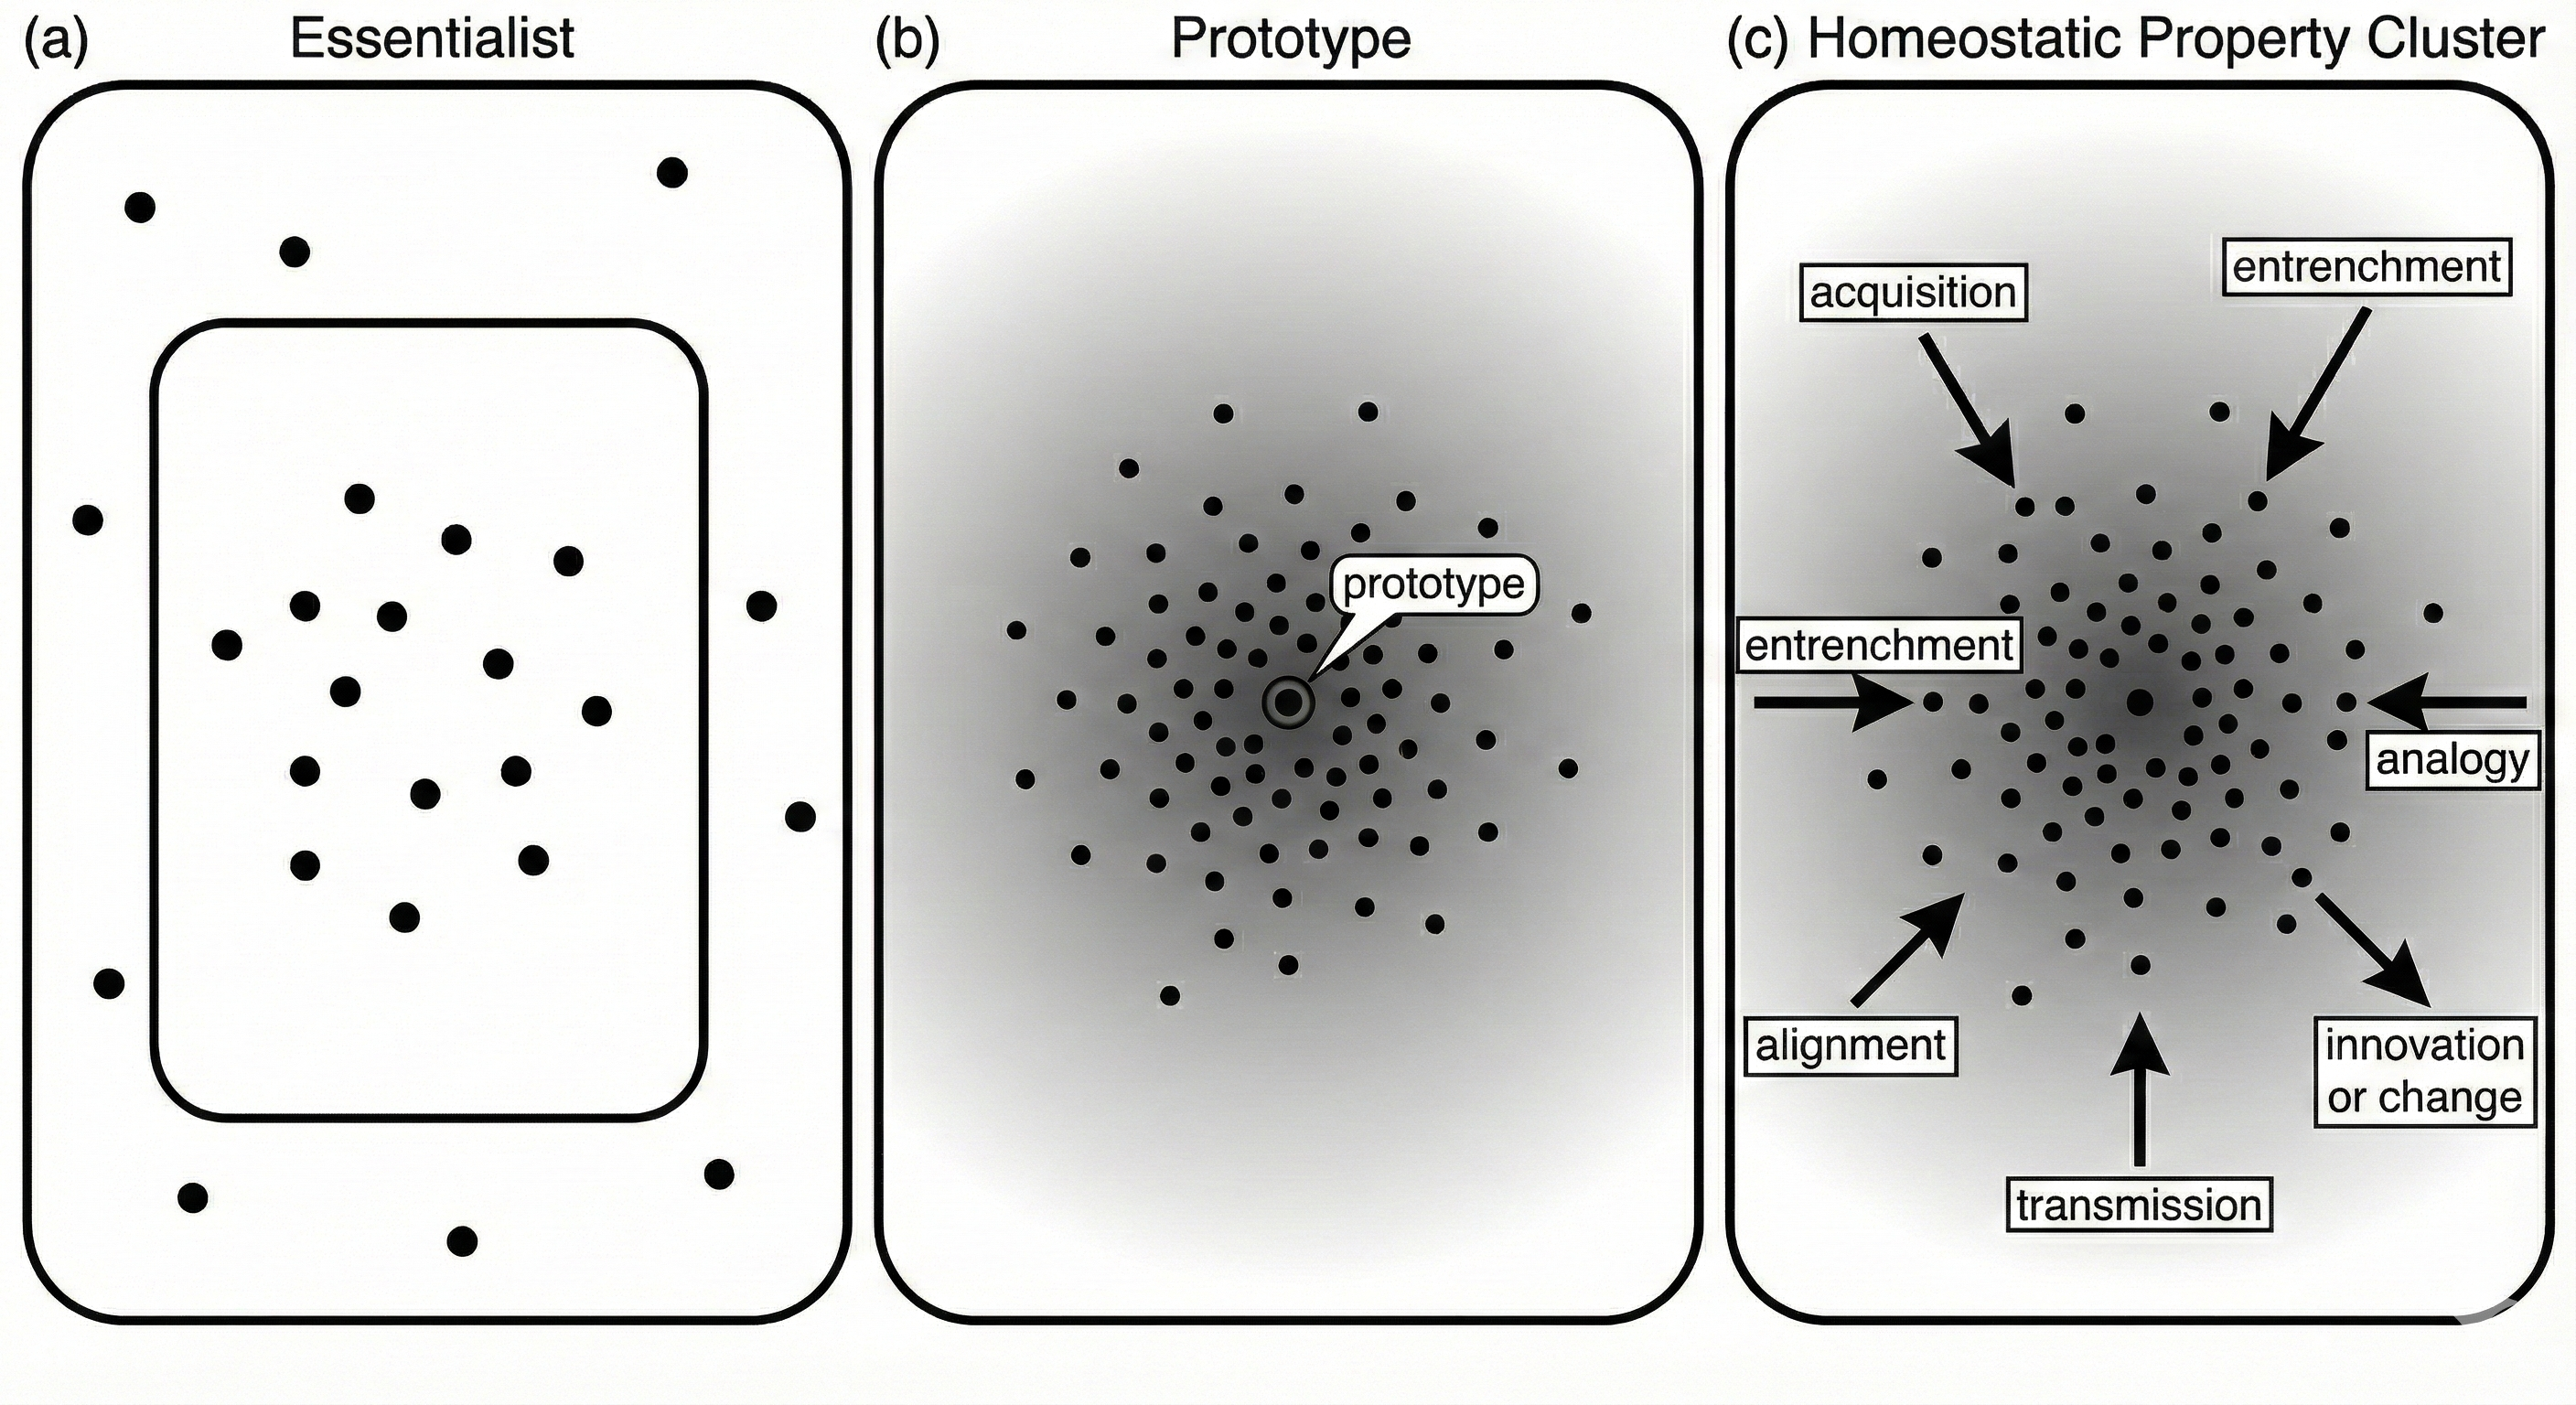
\includegraphics[width=\textwidth]{figures/1.1.png}
    \caption{Three conceptions of a category. (a)~The essentialist view: membership is determined by necessary and sufficient conditions; boundaries are sharp. (b)~The prototype view: membership is graded by similarity to a central exemplar; boundaries are fuzzy but the gradience is descriptive, not explained. (c)~The HPC view: membership is graded, and the cluster is maintained by identifiable causal mechanisms—acquisition, entrenchment, analogy, alignment, and transmission. The gradience in (c) is not merely observed but predicted by the theory.}
    \label{fig:three-conceptions}
\end{figure}

None of these mechanisms is unique to nouns or to lexical categories generally. They apply across linguistic structure: to phonemes and prosodic units, to inflectional classes and derivational patterns, to phrase types and grammatical relations, to construction families and discourse markers, to thematic roles and speech acts~-- to any category maintained across a population of speakers and transmitted over time. And none of them requires an essence.\footnote{A natural worry: aren't grammatical categories just conventions, like money or national borders? The answer is no~-- or rather, not in the way that matters. Conventions exist because we collectively treat them as existing; grammatical categories exist because causal mechanisms maintain them, whether or not anyone explicitly recognises those mechanisms. The distinction between purely institutional kinds (which depend on collective intentionality) and causal social kinds (which depend on causal structure) will be developed in Chapter 8. For now, the key point is that grammatical categories behave like the latter: they have discoverable structure that resists arbitrary redefinition.} They're causal processes that operate on populations of linguistic units, producing and maintaining the clustering that grammarians describe.

These mechanisms are not new. Usage-based and constructionist frameworks have been developing them for decades: Bybee on entrenchment and analogy, Tomasello on acquisition, Pickering and Garrod on alignment, Kirby on iterated learning. What the HPC framework adds is not the mechanisms themselves but three things: first, an explicit connection to the philosophy of science literature on natural kinds, which clarifies the ontological status of the categories these mechanisms maintain; second, principled criteria for distinguishing genuine kinds from mere family-resemblance clusters (developed in Chapter 8); and third, an explanation of why prototype effects arise as predictable consequences rather than unexplained primitives. The machinery is shared; the theoretical interpretation differs.

\begin{figure}[ht]
    \centering
    \includegraphics[width=0.85\textwidth]{figures/1.2.png}
    \caption{The mechanism cycle. Grammatical categories are maintained by a continuous feedback loop: usage events provide input to learners, who extract and entrench patterns; speakers align with interlocutors, reinforcing shared structure; entrenched patterns are transmitted to the next generation of learners, whose usage events continue the cycle. The stable category cluster (centre) is the emergent outcome of this process, not a static object but a dynamic equilibrium sustained by ongoing linguistic activity.}
    \label{fig:mechanism-cycle}
\end{figure}

\subsection*{What this explains}

Return to the cases that opened the chapter.

\mention{Otherwise} sits at the intersection of categories. It's adverb-like in some constructions, preposition-like in others, adjective-like in still others. Huddleston's puzzle~-- what \emph{is} it?~-- presupposes that it must be something, one thing. The HPC view says: it's subject to mechanisms that maintain adverb properties in some contexts, preposition properties in others, adjective properties in still others. The boundaries between these categories are zones where the mechanisms compete, and \mention{otherwise} lives in that zone. Its instability isn't a failure of analysis. It's a reflection of the causal structure. We must distinguish the difficulty of description from the nature of the thing described, but here the descriptive impasse tracks the causal reality. The classification struggle reflects the mechanism competition, rather than being a mere artifact of our categories.

Consider \mention{worth}. It looks like an adjective: it takes degree modifiers (\mention{well worth it}, \mention{hardly worth the effort}) and functions only predicatively. But it behaves like a preposition: it takes noun-phrase complements (\mention{worth ten dollars}) and cannot be used attributively (\mention{*a worth book}). Yet it resists the fronting that prepositions allow (\mention{*worth how much is it?}). This mix of properties led \citet{maling1983} to reanalyze it as a preposition, while others insist it remains an adjective. The dispute has lasted decades because the criteria themselves conflict. On the HPC view, \mention{worth} is caught in a tug-of-war: subject to the predicative licensing mechanisms of adjectives but the complement-selection mechanisms of prepositions, while lacking the movement properties of either. It occupies a stable niche where these forces balance, creating a category profile that is unique but perfectly explicable in terms of the intersecting mechanisms that maintain it. The \enquote{toxic disagreement} is just the sound of mechanisms clashing.

\mention{Cattle} is a noun, but a marginal one. It has plural agreement, takes numerals, heads noun phrases~-- but lacks the singular–plural contrast that prototypical nouns have. On the essentialist view, this is a problem: either \mention{cattle} is a noun or it isn't, and if it is, it should have noun properties. On the prototype view, \mention{cattle} is simply distant from the prototype~-- but then why this particular distance, this particular profile, stable for five hundred years?

On the HPC view, \mention{cattle} has just the kind of profile you'd expect for an item partially but not fully subject to the mechanisms that maintain nounhood. It's entrenched in noun-phrase constructions: \mention{the cattle}, \mention{these cattle}, \mention{many cattle}. That entrenchment maintains its nominal properties. But it lacks a singular form, which means it's not subject to the full paradigmatic pressure that shapes regular nouns. The mechanisms that would give it a singular~-- analogy to \mention{dog/dogs}, \mention{cat/cats}~-- have never taken hold. The clustering is partial because the mechanism application is partial. And it's stable because the pressure to regularize is relieved by a functional anchor: the word \mention{cow} is available to pick out individual animals. With \mention{cow} handling the singular function, \mention{cattle} is free to remain an aggregate, entrenched in its partial cluster \citep{reynolds2025countability}.

More generally, intersection zones between major categories are precisely the chronic trouble spots the framework predicts.

The adjective–adverb border is chronically unstable. Words drift across it; diagnostics conflict; grammarians disagree. On the HPC view, this is predicted: the mechanisms that maintain adjective clustering and the mechanisms that maintain adverb clustering overlap substantially. Both categories contain modifiers; both tolerate degree marking; both can appear predicatively. Where the mechanisms overlap, the boundary is weak. Where they diverge (adjectives modify nouns; adverbs modify verbs and clauses), the boundary has more force. The fuzziness has a shape, and the shape reflects the mechanisms. But this raises a question the framework must answer: when do overlapping mechanisms yield a genuine kind, and when do they yield merely a convenient fiction~-- a family-resemblance cluster with no real unity? The adjective–adverb boundary might be weak not because two robust kinds happen to overlap, but because there is no single kind there at all. Chapter 8 develops criteria for making this distinction.

\begin{figure}[ht]
    \centering
    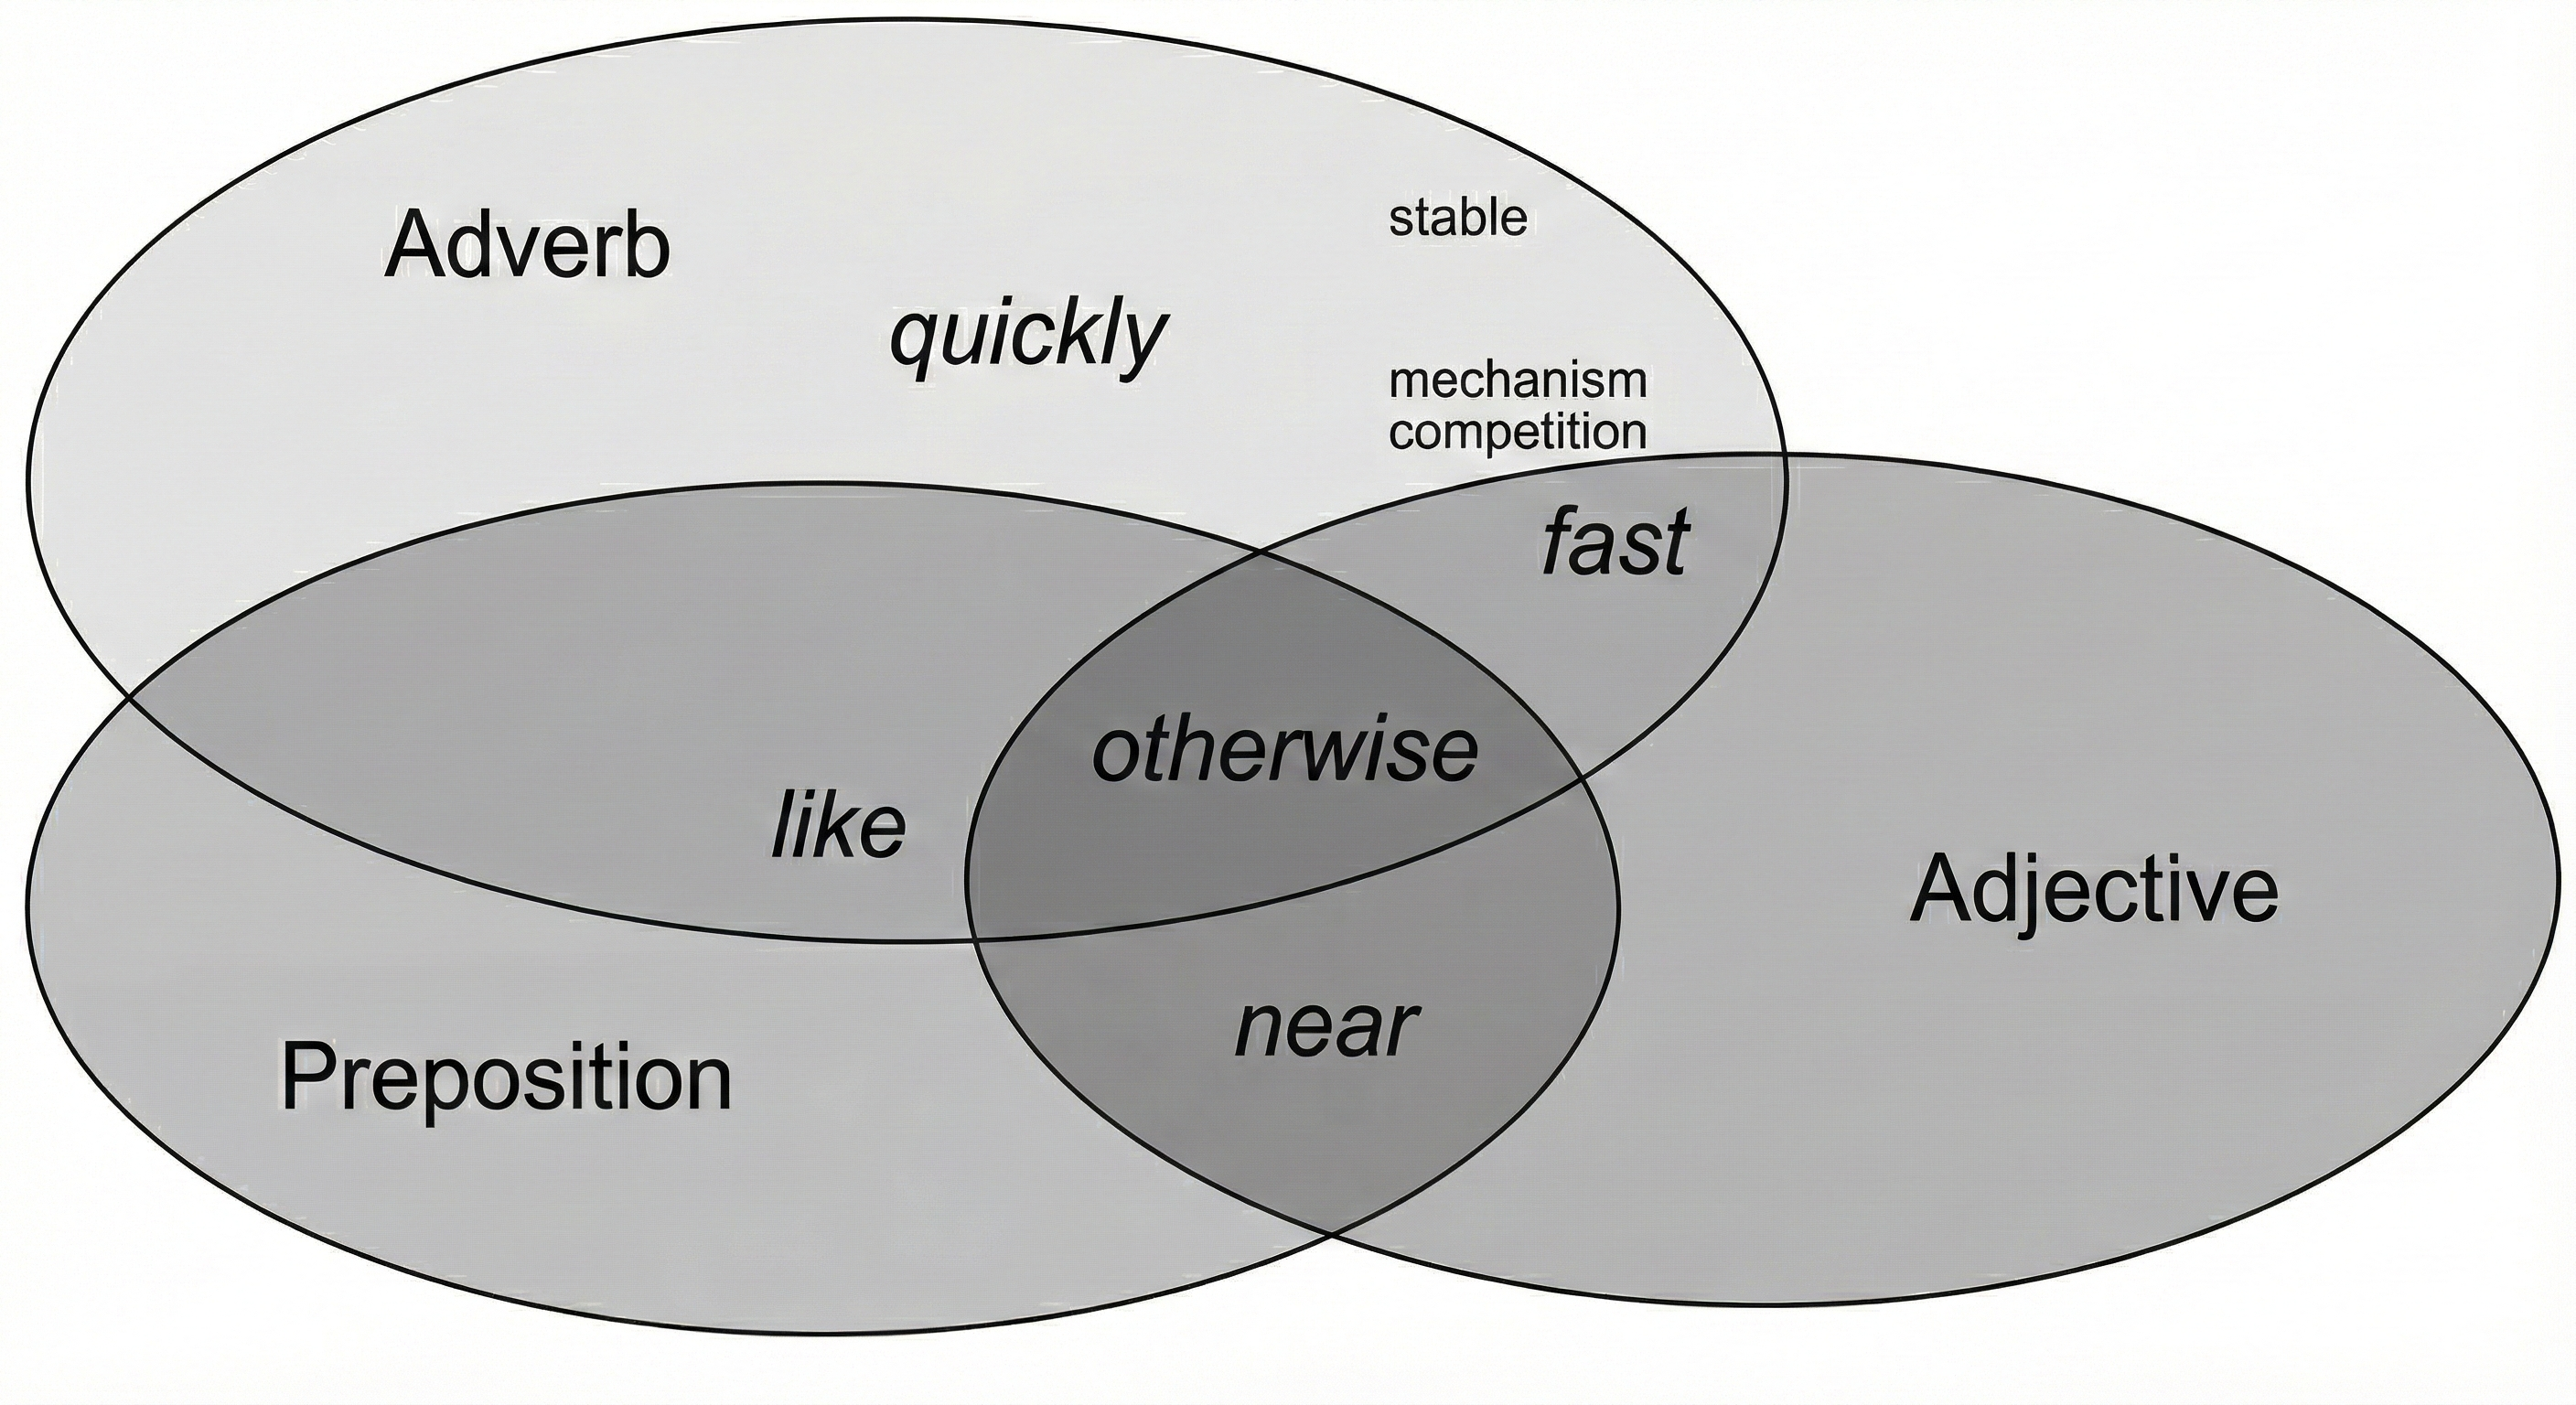
\includegraphics[width=0.85\textwidth]{figures/1.3.png}
    \caption{Boundary competition among three word classes. Words like \textit{quickly} sit firmly within a single category, subject to a consistent set of maintaining mechanisms. Words like \textit{fast} and \textit{like} occupy zones where two categories overlap—where mechanisms compete but one dimension of contrast is neutralised. Words like \textit{otherwise} and \textit{near} sit in the triple-overlap zone, subject to pulls from all three categories depending on construction and context. The instability of such items is not an analytical failure but a predictable consequence of the HPC framework: where mechanisms compete, category membership is genuinely contested.}
    \label{fig:boundary-competition}
\end{figure}

The noun–verb boundary is firmer. Not because nounhood and verbhood have sharper essences, but because the mechanisms that maintain them diverge more strongly. Nouns and verbs differ in argument structure, inflectional paradigms, syntactic distribution, constructional environments. The clustering forces pull in different directions. Items do cross the boundary, but usually by giving rise to distinct, though related, lexemes (verb \mention{run}, noun \mention{run}), rather than by hovering indefinitely in a single indeterminate space.

\bigskip

A natural question: if these mechanisms are language-particular and externalist~-- operating on populations of speakers rather than being innate to the language faculty~-- why do unrelated languages converge on broadly similar category inventories? The answer is that the mechanisms themselves are shaped by shared constraints. Processing efficiency favours category structures that minimise dependency lengths and memory load \citep{gibson2019efficiency}. Iterated transmission favours structures that are learnable by children with limited data \citep{kirby2015compression}. Communicative pressure favours structures that balance expressiveness against ambiguity. These constraints are not linguistic universals in the Chomskyan sense; they're cognitive, communicative, and information-theoretic pressures that any language must satisfy. Similar pressures produce similar solutions. The convergence is real, but it's explained by shared external constraints on language evolution, not by an innate inventory of categories.

\subsection*{Prototype effects, reconsidered}

I said earlier that prototype effects become shadows cast by deeper causal structure. Here's what that means.

On the prototype view, typicality is explanatorily basic. \mention{Dog} is a prototypical noun; \mention{fun} is a marginal noun; the difference in typicality explains the difference in behaviour. But this gets the explanatory order backwards. Typicality judgments are \emph{consequences} of category structure, not causes of it.

\mention{Dog} is typical because it's fully subject to the mechanisms that maintain nounhood. It inflects for number; it takes determiners; it heads argument phrases; it's massively entrenched in nominal constructions. Speakers experience it as a clear noun because nothing about its behaviour deviates from the cluster. \mention{Fun} is marginal because it's only partially subject to those mechanisms: it doesn't pluralise (\mention{*funs}), it resists determiners in some contexts (\mention{*a fun}), it has adjective-like uses (\mention{a fun time}). Speakers experience it as an unclear noun because its behaviour deviates from the cluster in systematic ways.

The prototype is an epistemic summary of the cluster. It's what speakers extract from their experience of the category. But the cluster itself is maintained by mechanisms, and the mechanisms explain both the prototype and the deviations from it. Prototype effects don't disappear on the HPC view. They're relocated: from the foundation of the account to a predictable consequence of it.

\subsection*{What comes next}

The HPC framework gives us a way to think about grammatical categories that accommodates the gradience, explains the stability, and generates predictions. But the framework is only as good as the mechanistic story that fills it in.

The rest of Part I sharpens the diagnosis. If essentialism could be saved by minor tweaks, someone would have saved it; Chapter 2 shows why the fixes fail. If prototype theory explained the stability, the problem would be solved; Chapter 3 shows why it doesn't. Chapter 4 counts the cost~-- research programmes in typology and theory that have stalled because the foundations won't bear weight.

Part II builds the alternative. What makes something an HPC kind (Chapter 5)? Why do such kinds support induction (Chapter 6)? What mechanisms maintain grammatical clusters (Chapter 7)? How do you know when you don't have a kind at all (Chapter 8)?

Part III applies the framework where it matters: countability, definiteness, word classes, and the rest of the grammatical stack from phonemes to constructions.

Part IV asks what follows~-- for grammaticality judgments, for linguistic methodology, for how the field should proceed.

The argument throughout will be that grammatical categories are real, stable, and explanatorily powerful~-- not because they have essences, but because mechanisms hold them together. The boundaries are genuinely fuzzy~-- not because categories are merely convenient fictions, but because mechanisms weaken, compete, and overlap. The fuzziness and the firmness have the same source.

\bigskip

Huddleston wrote, \enquote{I don't know how to handle} certain uses of \mention{otherwise}. The honest answer is that nobody does~-- not if \enquote{handling} means assigning a fixed category. But the HPC framework tells us why that's the wrong demand. \mention{Otherwise} sits where mechanisms compete, and the competition is the explanation. The word won't hold still because nothing's making it hold still. Understanding that's how to handle it.
